\documentclass{article}
\usepackage{pgfplots}
\usepackage{amsmath}

\begin{document}

\textbf{Buffer memory usage comparison.} Under $256 \times 256$, one transparent object buffer causes around 4.5 megabytes of memory. Our blending algorithm is summation based and thus do not require space to store each transparency buffer.

\begin{figure}[h]
    \centering
    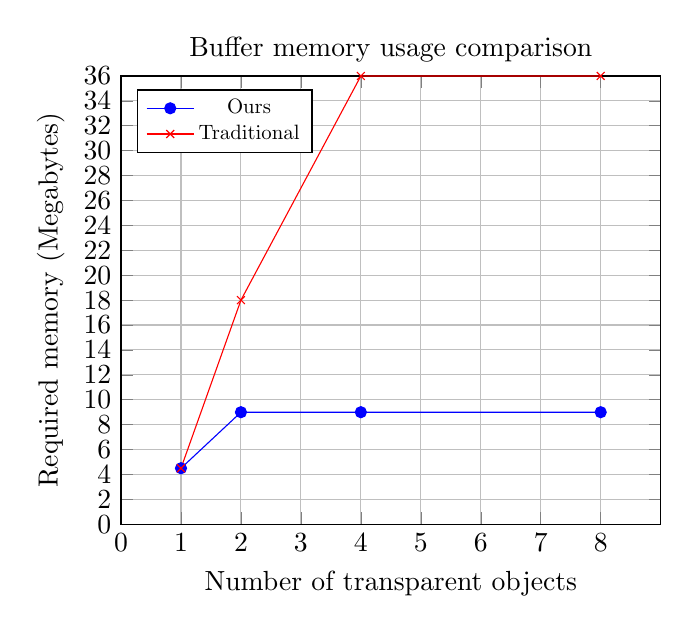
\begin{tikzpicture}
        \begin{axis}[
            xlabel={Number of transparent objects},
            ylabel={Required memory (Megabytes)},
            grid=major,
            legend pos=north west,
            ymin=0,
            ymax=36,
            xmin=0,
            xmax=9,
            ytick={0,2,...,36},
            xtick={0,1,...,8},
            title style={yshift=-1ex},
            title={Buffer memory usage comparison},
            legend style={nodes={scale=0.75, transform shape}},
            clip=false % Uncomment if needed
        ]
            \addplot [color=blue, mark=*] coordinates {
                (1, 4.5)
                (2, 9)
                (4, 9)
                (8, 9)
            };
            \addlegendentry{Ours}
            
            \addplot [color=red, mark=x] coordinates {
                (1, 4.5)
                (2, 18)
                (4, 36)
                (8, 36)
            };
            \addlegendentry{Traditional}
        \end{axis}
    \end{tikzpicture}
    \caption{Buffer memory usage comparison between our method and the traditional method.}
    \label{fig:buffer_memory_comparison}
\end{figure}

\end{document}